\chapter{Result and Discussion} \label{chp:result_and_discussion}

The performance of GBM will be evaluated by means of a case study using the test dataset. The test dataset comprises journey data from the whole year of 2021. The first part will focus on performance evaluation of BBM, where the trained model will be used to predict the SOG. The second part focus on the power estimation method using Holtrop-Mennen method. The output of BBM, which is the ship SOG, will be fed to the WBM to estimate the power. For further clarity regarding the methodology, the following steps are taken which are based on the proposed methodology shown in \Cref{fig:flowchart_BBM} and \Cref{fig:flowchart_WBM}. For generation of the BBM, the steps taken are:

\begin{enumerate}
    \setlength\itemsep{0em}
    \item Dataset is loaded.
    \item Identify and remove any anomalies.
    \item Remove static and unneeded features.
    \item Apply speed threshold of 5 knots.
    \item Highly correlated features are combined/removed based on physical and statistical reasoning.
    \item Impute missing values using {\tt KNNImputer}.
    \item Split the dataset into training and testing.
    \item Train the model using the whole dataset with default hyperparameter.
    \item Evaluate model performance using k-fold cross-validation.
    \item Tune the model until the best model is obtained.
    \item For the case study, the best models will be used to predict the SOG using the test dataset.
\end{enumerate}

Subsequently, for FOC calculation, the following steps are taken:

\begin{enumerate}
    \setlength\itemsep{0em}
    \item The test dataset is split into seasonal data. Summer-Fall season and Winter-Spring season which correspond to data for 6 months respectively.
    \item Impute missing values using {\tt KNNImputer}.
    \item SOG is converted to STW.
    \item Calculate calm water resistance $R_{CALM}$.
    \item Calculate added resistance due to wave $R_{AW}$.
    \item Calculate added resistance due to wind $R_{AA}$.
    \item Calculate total effective power $P_E$ using total resistance $R_{TOTAL}$.
    \item Calculate brake power $P_B$ from total efficiencies.
    \item Plot resulting regression line for Power-Speed curve from all models and actual case. 
    \item Calculate the FOC by considering the engine SFOC and operation time.
    \item Plot resulting regression line for FOC-Speed curve from all models and actual case.
    \item Evaluate the performance of the model generated from the regression lines.
\end{enumerate}

\section{Evaluation of BBM}\label{sec:BBM_tree_evaluate}

\subsection{Model Training and Selection of Optimal Parameter}\label{sec:hpo_select_train}

As mentioned in \Cref{sec:BBM_modelling}. There are 2871 data points available for training. To help narrow the search range of the hyperparameters for the tree-based model, RMSE plots against different values of hyperparameters will be performed. This method was presented in \Cref{sec:hpo}. The hyperparameter will be iteratively tuned until the best model is obtained. The result of the optimal parameter is found in \Cref{tbl:hpo_optimal}. The model training is executed using \textbf{AMD Ryzen 7 2700X, Eight-Core Processor $@$ 3.7 GHz processor with 16384 MB installed RAM}.\\


\begin{table}[ht]
    \footnotesize
    \centering
    % \resizebox {\textwidth}{!}
    {\begin{tabular}{ p{0.1\linewidth} p{0.2\linewidth}  p{0.3\linewidth} p{0.25\linewidth}}
    \hline
    Model & Training time [s] &  Optimal Hyperparameter & Search Range \\
    \hline
    DTR & 0.044 & None \\
    $\text{DTR}_{OPT}$ & 0.021  & {\tt min\_samples\_split = 7} & [2,10] \\
    &&{\tt min\_samples\_leaf = 10} & [1,10] \\
    &&{\tt max\_features = 12} & [1,12]\\
    &&{\tt max\_depth = 8} & [1,10] and [None]\\
    RFR & 4.112 & None \\
    $\text{RFR}_{OPT}$ & 3.431  & {\tt min\_samples\_split = 2} & [2,10]\\
    &&{\tt min\_samples\_leaf = 1} & [1,10]\\
    &&{\tt max\_features = 10} & [6,12]\\
    &&{\tt max\_depth = 120} & [10,200] and [None]\\
    &&{\tt n\_estimators = 100} & [100,1000]\\
    ETR & 0.944 & None \\
    $\text{ETR}_{OPT}$ & 4.390  & {\tt min\_samples\_split = 9} & [1,10]\\
    &&{\tt min\_samples\_leaf = 1} & [1,10]\\
    &&{\tt max\_features = 12} [1,12]\\
    &&{\tt max\_depth = 120} & [10,200] and [None]\\
    &&{\tt n\_estimators = 800} & [100,1000]\\
    MLR & 0.004  & None\\
    \hline
    \end{tabular}}
\caption{Optimal hyperparameter with training time of each model}\label{tbl:hpo_optimal}
\end{table}

With the default hyperparameter, RFR takes the longest training time followed by ETR and DTR. This is expected as RFR uses greedy algorithm i.e. it looks for the best possible feature when splitting the node. ETR takes significantly shorter time to train as ETR randomly select for features when splitting the node. DTR takes the shortest training time as it only generates a single tree. However, in the case of optimised model, ETR takes a longer time to train compared to RFR. This is caused by the number of trees in the optimised model which is controlled by the parameter {\tt n\_estimator}, the optimised ETR model has 800 trees in comparison to 100 trees of RFR. It is also observed that the training time of optimised DTR model is halved as pruning the tree resulted in a simpler model to train. \\

To further investigate the effect of hyperparameter optimisation, the learning curve of each tree-based model is plotted. For DTR, generated model with default parameter will result in a model that heavily overfits the training data, which is evident from the large gap between the training error and validation error which indicated a high variance as shown in \Cref{fig:learn_curve_DTR_MAE}. Regularisation i.e. parameter tuning of the DTR model helps balance between bias and variance by trading off bias for variance. This is observed from the substantial reduction in the gap between the training and validation error from \Cref{fig:learn_curve_DTR_MAE}. Additionally, the learning curve indicates that the model performance can be improved by increasing the amount of data points as the MAE continue to decrease with increasing amount of data points.\\

\begin{figure}[h]
    \centering
        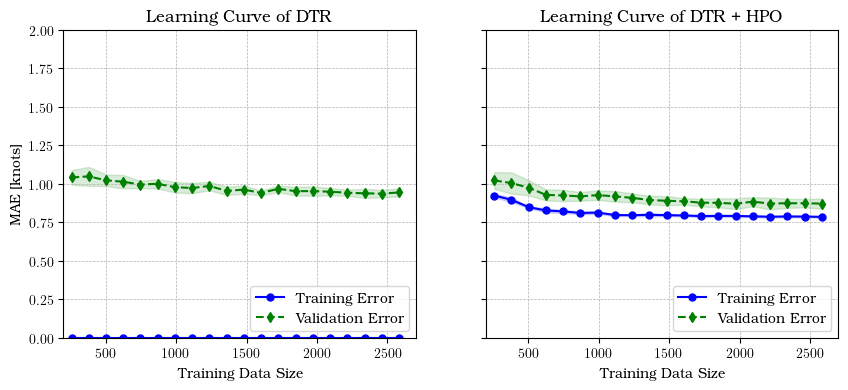
\includegraphics[width=.95\textwidth]{02_figures/learning_curve_dtr_mae.png}
        \caption{Learning curve of DTR}
        \label{fig:learn_curve_DTR_MAE}
\end{figure}

The process of hyperparameter tuning for the Random Forest Regressor (RFR) model did not show any significant improvement in model performance. This outcome aligns with the findings of  \bcitet{Kuhn.2013} and \bcitet{Hastie.2009} which was discussed in \Cref{sec:rf_theo}. The model starts to plateau at approximately 1000 data points. Furthermore, there is noticeable variance in the RFR model, which indicates that the model will have a slight tendency to overfit.\\

\begin{figure}[h]
    \centering
        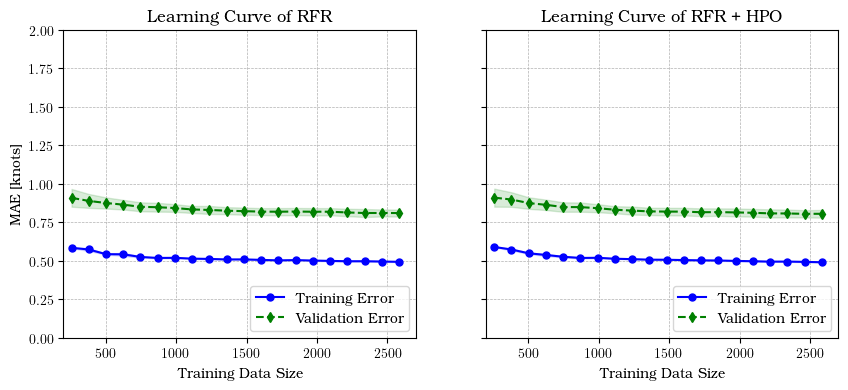
\includegraphics[width=.95\textwidth]{02_figures/learning_curve_rfr_mae.png}
        \caption{Learning curve of RFR}
        \label{fig:learn_curve_RFR_MAE}
\end{figure}

Hyperparameter tuning helps to reduce variance in the ETR model. But it does not have any major impact on model's performance. The ETR model reaches plateau beyond 1000 data points. Suggesting that adding more data points will not result in any tangible increase in model performance.\\

\begin{figure}[h]
    \centering
        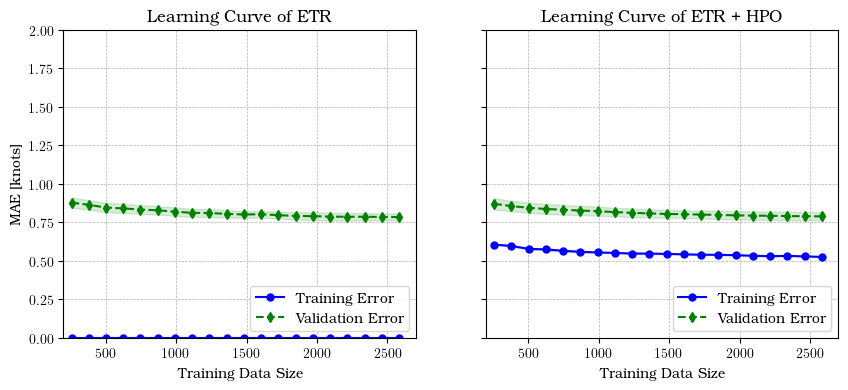
\includegraphics[width=.95\textwidth]{02_figures/learning_curve_etr_mae.png}
        \caption{Learning curve of ETR}
        \label{fig:learn_curve_ETR_MAE}
\end{figure}

\subsection{Analysis of trained model}\label{sec:BBM_model_eval}

\subsubsection{Feature Importance}\label{sec:feature_importance_bbm}

As discussed in \Cref{sec:rf_theo}, tree-based models are able to quantify the impact of each feature during the split process, this is performed using {\tt feature\_importances\_} feature in \scikit/ \bcitep{Kuhn.2013}. According to documentation by \bcitet{FabianPedregosa.2011}, it is computed as the mean and the standard deviation of accumulation of the impurity decrease within each tree i.e. total reduction of the criterion brought by a feature. Alternatively, it can be defined as how much a feature is used in each tree.\\

\begin{table}[ht]
    \scriptsize
    \centering
    \resizebox {\textwidth}{!}
    {\begin{tabular}{ p{0.15\linewidth} c| p{0.15\linewidth} c| p{0.15\linewidth} c}
    \hline
    $\text{DTR}_{OPT}$ & & $\text{RFR}_{OPT}$ & & $\text{ETR}_{OPT}$\\
    \hline
    Feature & Importance & Feature & Importance & Feature & Importance\\
    \hline
    {\tt heading} & 0.6563 & {\tt heading} & 0.4927 & {\tt cog} & 0.6410 \\
    {\tt cog} & 0.3183 & {\tt cog} & 0.4183 & {\tt heading} & 0.2707 \\
    {\tt draught} & 0.0105 & {\tt draught} & 0.0210 & {\tt truecurrentdir} & 0.0200\\
    {\tt truewinddir} & 0.0047 & {\tt curspeed} & 0.0104 & {\tt draught} & 0.0144 \\
    {\tt oceantemperature} & 0.0029 & {\tt waveperiod} & 0.0093& {\tt windwaveswellheight} & 0.0112\\
    {\tt surftemp} & 0.0025&{\tt truecurrentdir} & 0.0092 & {\tt curspeed} & 0.0110\\
    {\tt waveperiod} & 0.0019 & {\tt windwaveswellheight} & 0.0084& {\tt waveperiod} & 0.0095 \\
    {\tt truecurrentdir} & 0.0010 & {\tt surftemp} & 0.0075& {\tt windspeed} & 0.0053\\
    {\tt windwaveswellheight} & 0.0008 & {\tt truewinddir} & 0.0075& {\tt surftemp} & 0.0046 \\
    {\tt curspeed} & 0.0004 & {\tt truewavedir} & 0.0058& {\tt truewavedir} & 0.0045 \\
    {\tt windspeed} & 0.0004 & {\tt oceantemperature} & 0.0057& {\tt oceantemperature} & 0.0044\\
    {\tt truwavedir} & 0.0001 & {\tt windspeed} & 0.0056& {\tt truewinddir} & 0.0033\\
    \end{tabular}}
\caption{Feature importance of different models}\label{tbl:feature_importances}
\end{table}

The feature importances for all tree-based models shown in \Cref{tbl:feature_importances} indicated that the structure of the model is significantly influenced by the features {\tt heading} and {\tt cog}. This finding indicated that the models predicted the SOG by basis of ship movement direction i.e. heading and COG for a particular location. However, in a physical sense, it will be more insightful to consider the ship state and weather conditions that affect the prediction of the SOG.\\

\begin{figure}[h]
    \centering
        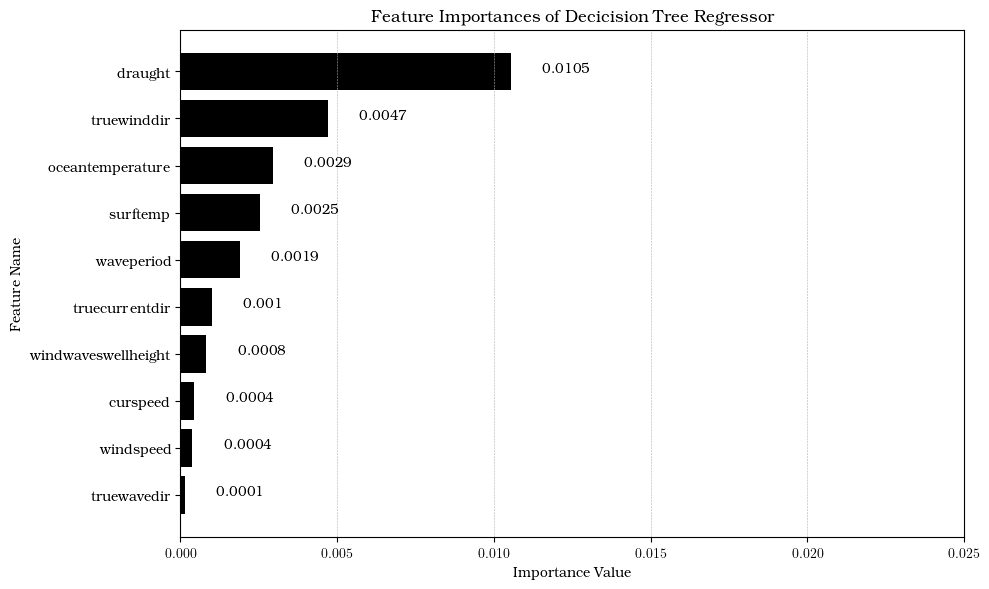
\includegraphics[width=.9\textwidth]{02_figures/dtr_ftr_importance_nodir.png}
        \caption{Feature importance of DTR}
        \label{fig:ftr_impo_dtr}
\end{figure}

Excluding ship heading and COG. The ship draught $T$ is regarded as the significant factors that affect the SOG prediction. This aligns with the theory of frictional resistance $R_F$ encountered by the ship, which is discussed in \Cref{sec:Calm_Resistance}. \Cref{eqn:R_f} is a function of wetted surface area of bare hull $S$. Deeper draught $T$ will result in more submerged area of the hull and this will consequently increase the frictional force $R_F$ of the ship. Given a constant supply of power to the ship propulsion system, the speed of the ship will decrease which is shown in \Cref{eqn:P_e}.\\

\begin{figure}[h]
    \centering
        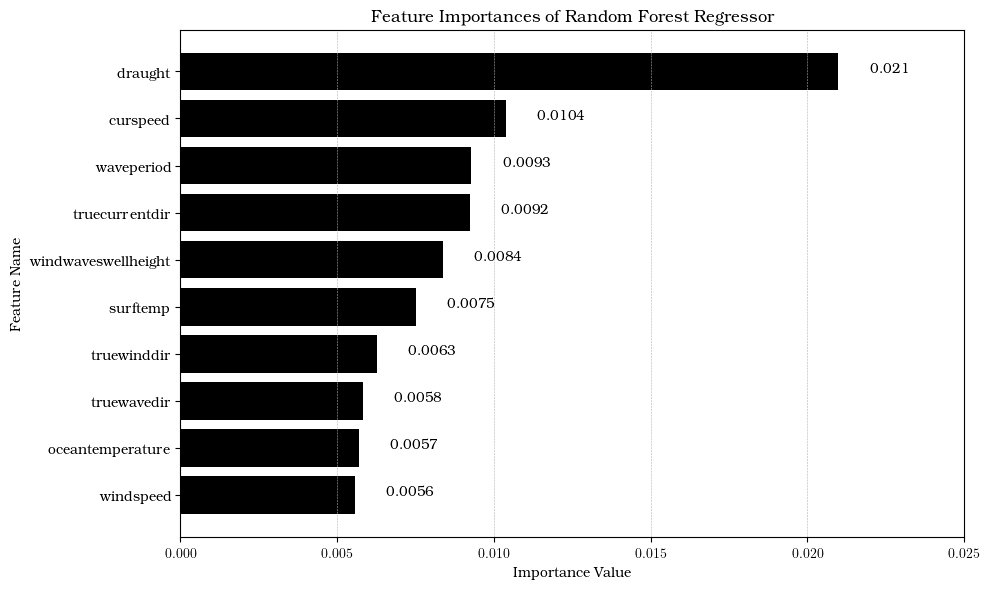
\includegraphics[width=.9\textwidth]{02_figures/rfr_ftr_importance_nodir.png}
        \caption{Feature importance of RFR}
        \label{fig:ftr_impo_rfr}
\end{figure}

\begin{figure}[h]
    \centering
        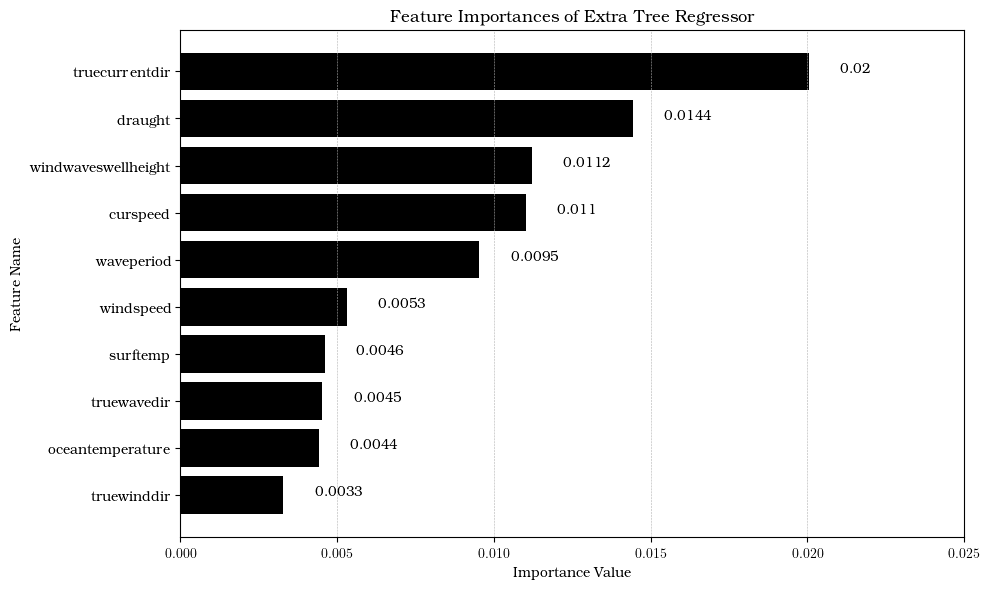
\includegraphics[width=.9\textwidth]{02_figures/etr_ftr_importance_nodir.png}
        \caption{Feature importance of ETR}
        \label{fig:ftr_impo_etr}
\end{figure}

For weather states, both RFR and ETR considered current based information such as current speed and true current direction as the most significant weather factor that affect SOG prediction. This aligns to the proposed current correction methodology presented in \Cref{sec:SOG_corr} which states that the process of current correction to convert SOG to STW requires both the magnitude and direction of the current. The next influencing feature ranked by RFR and ETR model are wave related features which are significant wave height $H_{1/3}$, true wave direction, and the wave period {\tt waveperiod}. This corresponds to the added resistance due to wave $R_{AW}$ in the calculation of total resistance $R_{TOTAL}$ encountered by the ship. The wind related features, which are wind speed and its true direction, corresponds to added resistance due to wind force $R_{AA}$ and is found to be the least influential in SOG prediction in RFR and ETR model.\\

Based on the behaviour of the Random Forest Regressor (RFR) and Extra Trees Regressor (ETR) models, it can be inferred that waves have a more significant impact on the Speed Over Ground (SOG) compared to the influence of wind during the ship's journey. However, the Decision Tree Regressor (DTR) model demonstrates that temperature-related features, such as Sea Surface Temperature (SST) and air temperature above the ocean, have a more significant effect on SOG predictions than most other features. While the importance of temperature is not as pronounced as in RFR or ETR models, this finding suggests that the ship's SOG is implicitly influenced by the time of the travel or the season in which the journey takes place.\\

\subsubsection*{Structure of generated tree-based model}

\begin{figure}[h]
    \centering
        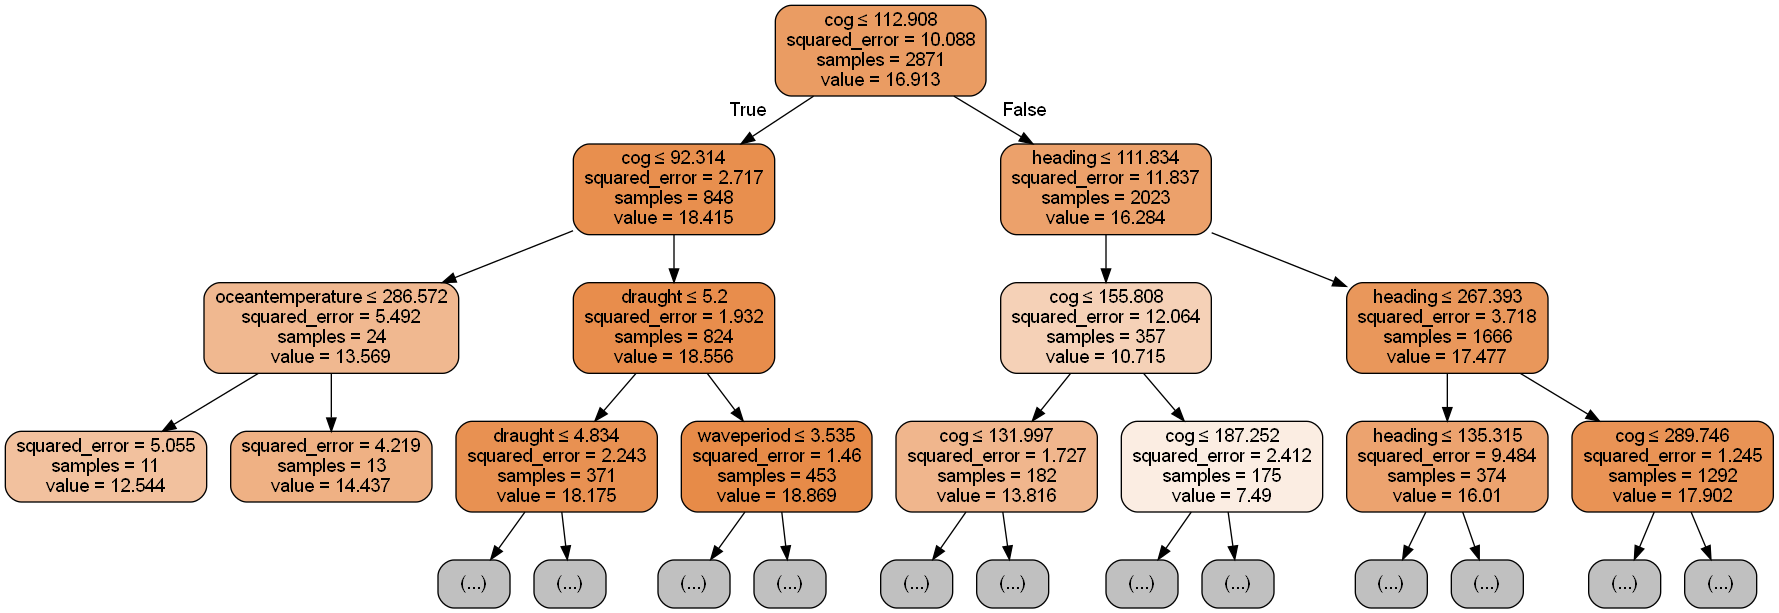
\includegraphics[width=.9\textwidth]{02_figures/dtr_mod_1tree.png}
        \caption{Partial structure of DTR}
        \label{fig:dtr_tree_hpov}
\end{figure}

To understand the effect of hyperparameter optimisation and feature importance, analysis on the structure of generated tree-based models will be performed. The shading in the nodes indicated the likelihood of the decision, where darker shading means greater likelihood. Each node indicates information on the splitting feature with the threshold, the SSR score, amount of samples and the predicted SOG value. Even after pruning, the tree can grow relatively large, therefore, the illustration of the trees is limited to a depth of {\tt max\_depth = 3} and for RFR and ETR, only the illustration of a specific tree in the forest will be shown.\\

The structure of the optimised decision tree shown in \Cref{fig:dtr_tree_hpov} show the effect of regularisation at the leaf node. For example, the leaf nodes that splits the feature, ocean temperature, does not completely minimise the SSR. This is caused by the hyperparameter tuning of the minimum samples at the leaf node, which was set at {\tt min\_samples\_leaf = 10}, splitting these nodes further will cause subsequent leaf nodes that have less than 10 samples. In this figure, the significance of COG and ship heading can be clearly seen, as it is used to split many of the internal nodes in the tree.\\

\begin{figure}[h]
    \centering
        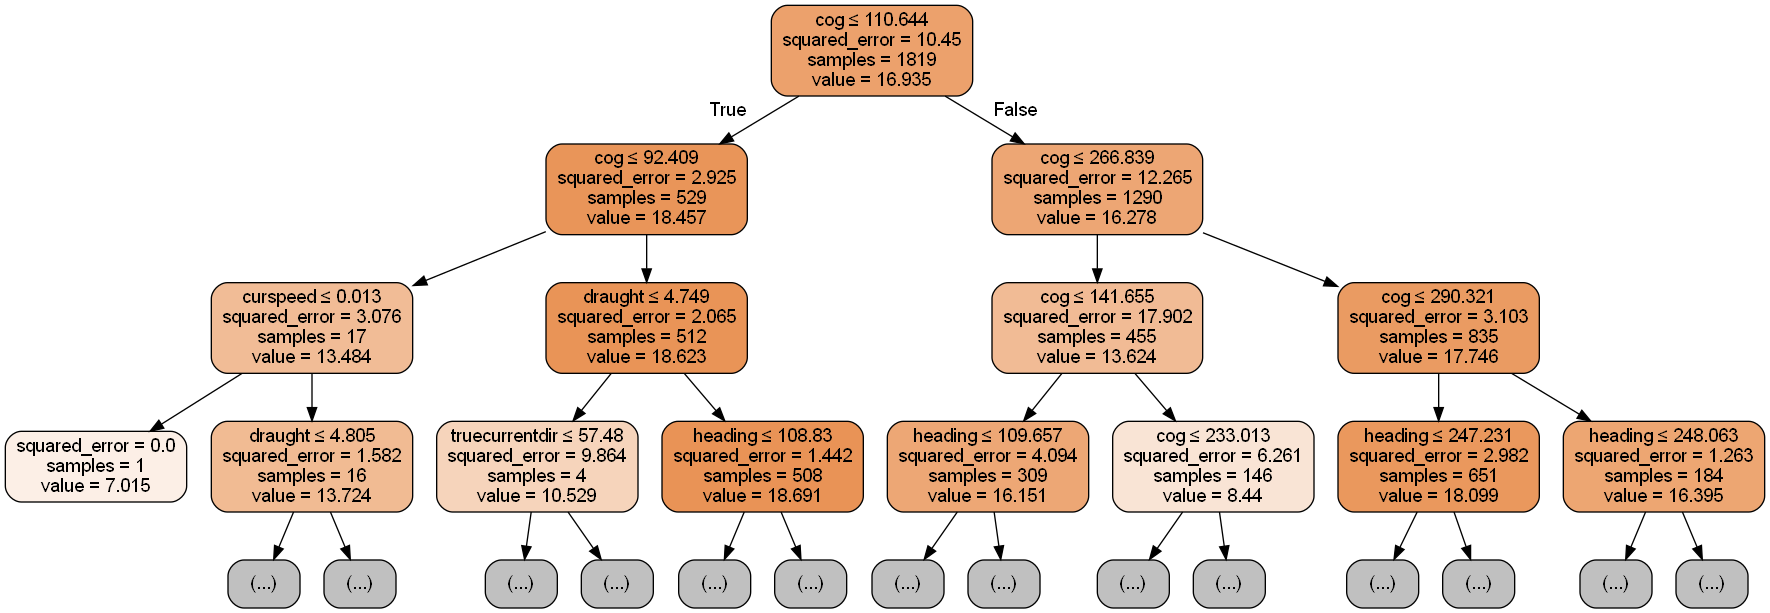
\includegraphics[width=.9\textwidth]{02_figures/rfr_mod_it1.png}
        \caption{Partial structure of {\tt n\_estimators = 1} for RFR}
        \label{fig:rfr_tree1_hpov}
\end{figure}

The illustration of the first RFR tree is shown in \Cref{fig:rfr_tree1_hpov}. Similar to DTR, both COG and ship heading are regarded as the best features to split the internal node. In this tree of the forest, the effect of allowing full tree growth can be observed in the leaf node when splitting the feature current speed. This tree is able to minimise the SSR to its possible minimum value, and the leaf node cannot be further split as there are no more available samples. The effect of bagging for the dataset and feature selection in RFR can also be observed in this tree as the structure of this tree is completely different to DTR tree shown in \Cref{fig:dtr_tree_hpov}.\\

\begin{figure}[h]
    \centering
        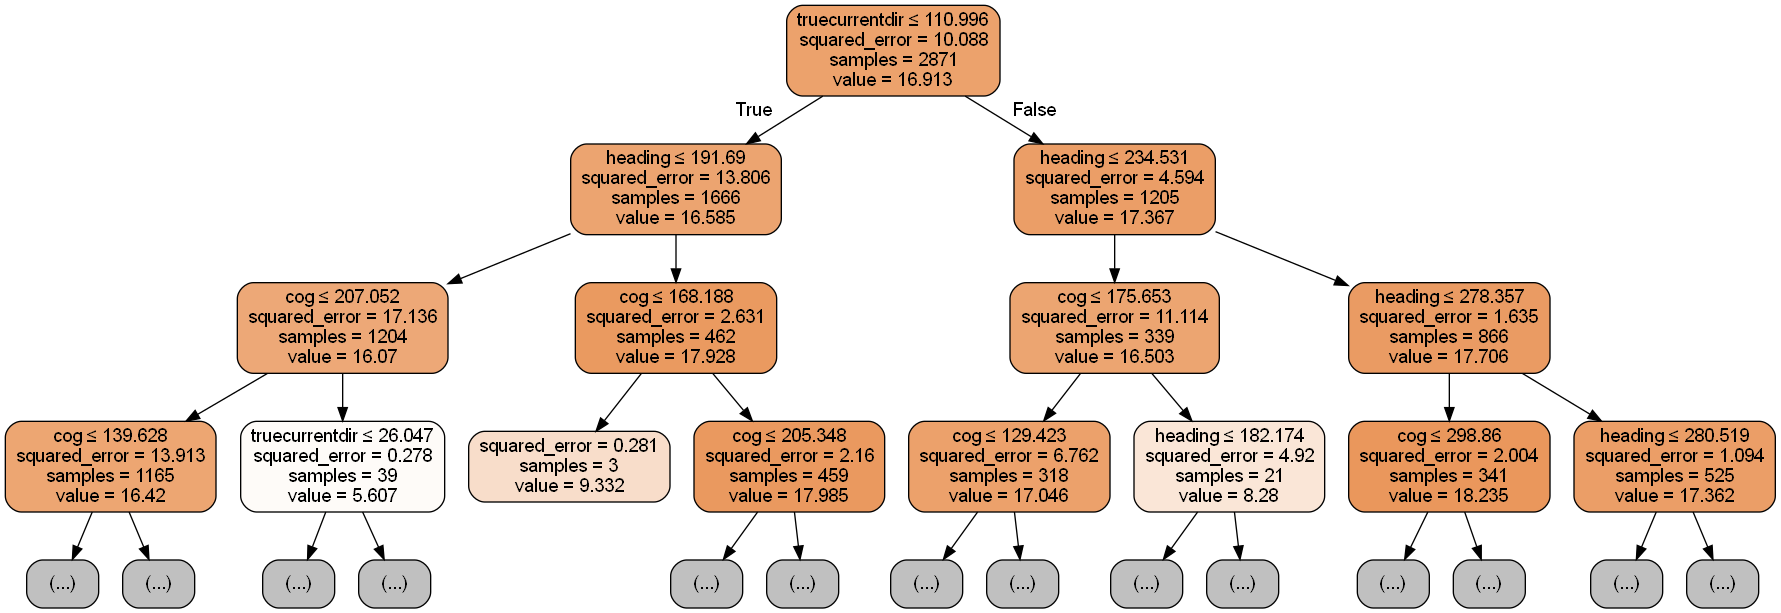
\includegraphics[width=.9\textwidth]{02_figures/etr_mod_it1.png}
        \caption{Partial structure of {\tt n\_estimators = 1} for ETR}
        \label{fig:etr_tree1_etr}
\end{figure}
The random selection of the feature to split of ETR can be seen in the structure of the first tree in an ETR in \Cref{fig:etr_tree1_etr}. Since both DTR and RFR uses greedy algorithm, i.e. it finds the possible splits which minimise the cost function, both model selected COG as the parent node. However, the randomness in feature selection of ETR can be clearly observed in this illustration, the model selects the true current direction as the parent node. Also, due to regularisation of ETR, the leaf node when splitting COG does not completely minimise the SSR. The split is not allowed since it does not meet the tuning criteria of {\tt min\_samples\_split = 9}.\\ 

\subsubsection{Evaluation of k-fold cross-validation}\label{sec:bbm_kfold_perf_eval}

The performance of the model is evaluated using the training dataset using 10-fold cross validation. This means that the training will be repeated 10 times using 9 of the folds as training dataset, the remaining fold will be used as validation dataset. The results from k-folding validation process is shown in \Cref{fig:k_fold_validation_result}. The inside (orange) line represents the median i.e. $50\%$ of the score in k-folding. The top and the bottom of the box correspond to the first i.e. $25\%$ and third quartile i.e. $75\%$ respectively. The whiskers represent the lowest data point within the 1.5 Interquartile Range (IQR) of the lowest quartile and the highest point of data within 1.5 IQR of the upper quartile. The mean is indicated by the (green) triangle. Data points beyond the whisker range is shown as hollow circle.\\
\begin{figure}[ht]
    \centering
  
    \begin{minipage}{0.45\textwidth}
      \centering
      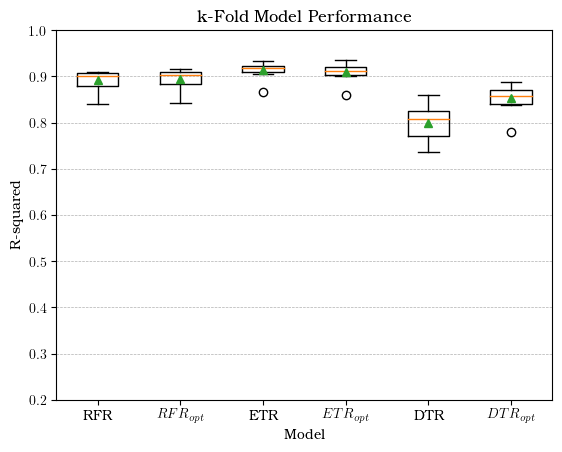
\includegraphics[width=\textwidth]{02_figures/kfold_r2_opt.png}
    \end{minipage}
    \hfill
    \begin{minipage}{0.45\textwidth}
      \centering
      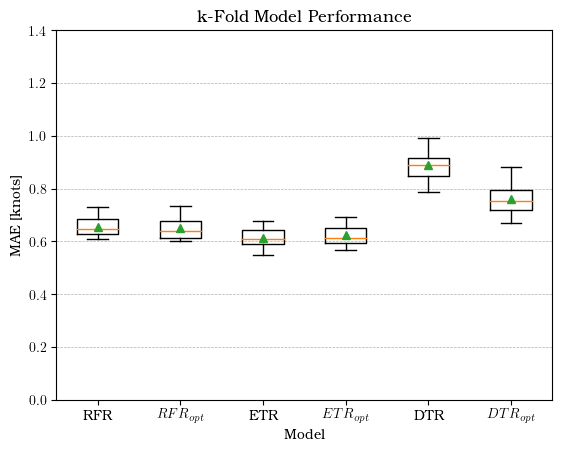
\includegraphics[width=\textwidth]{02_figures/kfold_mae_opt.png}
    \end{minipage}
  
    \vspace{0.5cm} % Adjust the vertical space between rows
  
    \begin{minipage}{0.45\textwidth}
      \centering
      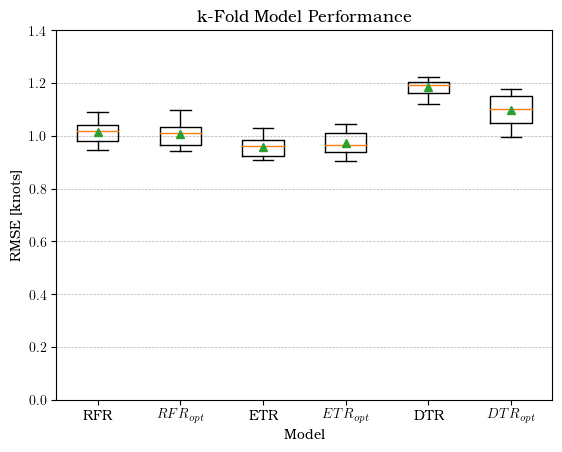
\includegraphics[width=\textwidth]{02_figures/kfold_rmse_opt.png}
    \end{minipage}
    \hfill
    \begin{minipage}{0.45\textwidth}
      \centering
      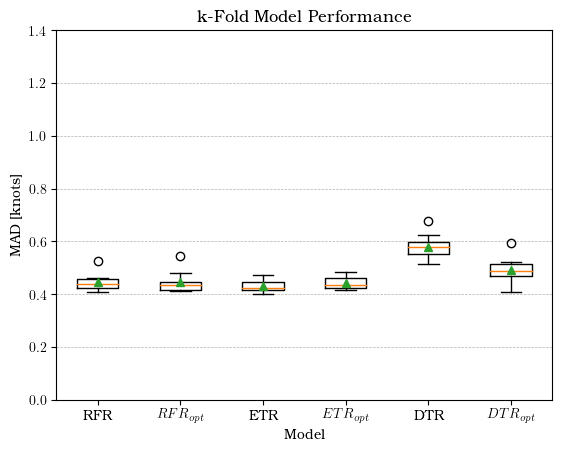
\includegraphics[width=\textwidth]{02_figures/kfold_mad_opt.png}
    \end{minipage}
  
    \caption{Evaluation of k-fold cross-validation for different performance indices}
    \label{fig:k_fold_validation_result}
  \end{figure}

The box plots indicated that ETR achieved the best performance, the model is able to achieve $R^2$ score of around $91\%$ and MAE of around 0.6 knots. The model is also relatively stable, which is indicated by the narrow box plots. RFR also achieved similar performance, achieving $R^2$ score of about $89\%$ and MAE of approximately 0.65 knots. As illustrated previously in \Cref{fig:learn_curve_ETR_MAE} and \Cref{fig:learn_curve_RFR_MAE}, optimisation does not yield any significant improvement in model performance. DTR greatly benefits from regularisation, the model achieves an increase of about $5\%$ for the $R^2$ score and a reduction from about 0.89 knots to 0.76 knots for the MAE, similar improvements can be observed in both RMSE and MAD. To summarise, all tree-based models exhibited good fit performance with mean/median $R^2$ scores above $80\%$. However, the value of RMSE is quite significant, the values lies between 1.00 to 1.20 knots across the models. To put this into scale, the mean SOG of the training data is at 16.91 knots as shown in \Cref{tbl:dataset_descriptive_pretraining}.\\  

\subsection{Performance evaluation of BBM}\label{sec:Perf_eval_BBM}

\subsubsection{Analysing the testing dataset}\label{sec:testing_data_analysis}

Once the best model is determined, the model will be tested against the testing dataset. The testing dataset correspond to 957 datasets across 2021, the dataset for the whole year is indicated as $DS_{year}$. To investigate the effect of data points on the model performance, the dataset is split into two seasons, $DS_{summer}$, which corresponds to summer datasets and it represents data between May 2021 and October 2021, there are 454 data points between this period. Winter dataset, $DS_{winter}$, correspond to testing datasets between January 2021 and April 2021 as well as November 2021 and December 2021 which correspond to 503 data points. Any missing values which are present in the testing dataset will be using {\tt KNNImputer}.\\

\begin{table}[h]
    \footnotesize
    \centering
    % \resizebox {\textwidth}{!}
    {\begin{tabular}{ p{0.21\linewidth} c c c c c c c c }
    \hline
    Features & Count & Mean & Std. & Min & 25\% & 50\% & 75\% & Max \\
    \hline
    \textbf{{\tt sog}} & 957.00 & 16.99 & 3.10 & 5.10 & 16.68 & 18.05 & 18.72 & 21.00\\
    \hline
    {\tt cog} & 957.00 & 196.73 & 86.72&	56.02 & 102.32& 185.22& 282.18& 319.85\\ 
    {\tt heading} & 957.00 & 188.30&	89.17&	63.49&	100.86&	124.24&	279.38&	308.04\\
    {\tt draught} & 957.00 & 5.23 & 0.19& 4.74& 5.11& 5.29& 5.38&5.66\\
    {\tt windspeed} & 957.00 & 6.45 & 3.04 & 0.40 & 4.11 & 6.13 &	8.21 & 15.85\\
    {\tt oceantemperature} & 957.00 & 282.28 & 6.48 & 267.25& 276.80& 281.91& 288.42& 295.70 \\
    {\tt waveperiod} & 957.00 & 3.70 & 0.88 & 1.67 & 3.06& 3.62& 4.22& 7.01\\
    {\tt surftemp} & 957.00 &283.22& 5.72& 273.15& 277.98& 282.73& 288.82 &294.93\\
    {\tt windwaveswellheight} &  957.00 & 0.77 & 0.54 & 0.08 &0.37 &	0.66 &	0.94 &  3.24  \\
    {\tt curspeed} & 957.00 &0.09 & 0.07& 0.00 & 0.05& 0.07 & 0.13 & 0.50\\
    {\tt truewinddir} & 957.00 & 91.39 & 56.23 &	0.03 & 38.80 &	95.25 & 142.83 & 179.86\\
    {\tt truecurrentdir} & 957.00 & 90.75 & 57.76 & 0.26 & 31.52 & 90.44 & 144.65 & 179.95 \\
    {\tt truewavedir} & 957.00 & 86.90 & 55.74& 0.06& 36.24 & 81.54 & 138.04 & 179.81 \\
    \hline
    \end{tabular}}
\caption{Descriptive statistics of $DS_{year}$}\label{tbl:testyear_dataset_descriptive}
\end{table}

\begin{table}[h]
    \footnotesize
    \centering
    % \resizebox {\textwidth}{!}
    {\begin{tabular}{ p{0.21\linewidth} c c c c c c c c }
    \hline
    Features & Count & Mean & std & Min & 25\% & 50\% & 75\% & Max \\
    \hline 
    \textbf{{\tt sog}} & 454.00 & 17.26 & 2.91 & 5.22 & 16.74 & 18.17 & 18.95 & 21.01\\
    \hline
    {\tt cog} & 454.00 & 196.06 & 87.55 &  56.02 & 102.80 & 182.79 & 282.03 & 319.85 \\ 
    {\tt heading} & 454.00 & 188.08 & 89.02 &  63.49 & 100.75 & 124.68 & 278.07 & 303.30 \\
    {\tt draught} & 454.00 &   5.30 &  0.17 &   4.74 &   5.20 &   5.29 &   5.38 &   5.66 \\
    {\tt windspeed} & 454.00 &   6.64 &  3.33 &   0.40 &   4.08 &   6.30 &   8.71 &  15.85 \\
    {\tt oceantemperature} & 454.00 & 285.59 &  5.90 & 269.27 & 282.90 & 286.70 & 290.04 & 295.70 \\
    {\tt waveperiod} & 454.00 & 3.73 &  0.99 &   2.02 &   2.95 &   3.60 &   4.36 &   7.01 \\
    {\tt surftemp} & 454.00 & 286.33 &  5.10 & 274.75 & 283.05 & 287.58 & 290.18 & 294.93 \\
    {\tt windwaveswellheight} & 454.00 &   0.82 &  0.63 &   0.08 &   0.36 &   0.67 &   1.02 &   3.24 \\
    {\tt curspeed} & 454.00 &   0.10 &  0.07 &   0.00 &   0.04 &   0.07 &   0.13 &   0.50 \\
    {\tt truewinddir} & 454.00 &  90.94 & 58.05 &   0.60 &  38.40 &  89.86 & 145.86 & 179.58 \\
    {\tt truecurrentdir} & 454.00 &  83.65 & 59.53 &   0.26 &  26.68 &  70.51 & 143.73 & 179.33 \\
    {\tt truewavedir} & 454.00 &  88.06 & 59.52 &   0.09 &  33.00 &  82.18 & 145.69 & 179.81 \\
    \hline
    \end{tabular}}
\caption{Descriptive statistics of $DS_{summer}$}\label{tbl:testsummer_dataset_descriptive}
\end{table}

\begin{table}[h]
    \footnotesize
    \centering
    % \resizebox {\textwidth}{!}
    {\begin{tabular}{ p{0.21\linewidth} c c c c c c c c }
    \hline
    Features & Count & Mean & std & Min & 25\% & 50\% & 75\% & Max \\
    \hline
    \textbf{{\tt sog}} & 503.00 & 16.75 & 3.24 & 5.10 & 16.59 & 17.98 & 18.61 & 20.70\\
    \hline
    {\tt cog} & 503.00 & 197.33 & 86.06 &  80.81 & 102.25 & 187.56 & 282.63 & 307.92 \\
    {\tt heading} & 503.00 & 188.50 & 89.39 &  89.22 & 100.87 & 123.92 & 280.05 & 308.04 \\
    {\tt draught} & 503.00 &   5.16 &  0.18 &   4.76 &   5.02 &   5.20 &   5.29 &   5.65 \\
    {\tt windspeed}& 503.00 &   6.28 &  2.76 &   0.43 &   4.12 &   6.05 &   8.01 &  14.35 \\
    {\tt oceantemperature} & 503.00 & 279.29 &  5.44 & 267.25 & 275.74 & 278.22 & 281.25 & 292.72 \\
    {\tt waveperiod} & 503.00 & 3.67 &  0.76 &   1.67 &   3.16 &   3.62 &   4.14 &   5.98 \\
    {\tt surftemp} & 503.00 & 280.41 &  4.71 & 273.15 & 277.23 & 278.68 & 282.68 & 292.85 \\
    {\tt windwaveswellheight} & 503.00 &   0.73 &  0.45 &   0.08 &   0.40 &   0.66 &   0.90 &   2.43 \\
    {\tt curspeed} & 503.00 &   0.09 &  0.07 &   0.00 &   0.05 &   0.08 &   0.12 &   0.42 \\
    {\tt truewinddir} & 503.00 &  91.81 & 54.61 &   0.03 &  39.66 &  97.92 & 140.20 & 179.86 \\
    {\tt truecurrentdir} & 503.00 &  97.16 & 55.40 &   1.44 &  41.92 & 102.12 & 145.34 & 179.95 \\
    {\tt truewavedir} & 503.00 &  85.86 & 52.13 &   0.06 &  39.44 &  81.22 & 132.49 & 178.30 \\
    \hline
    \end{tabular}}
\caption{Descriptive statistics of $DS_{winter}$}\label{tbl:testwinter_dataset_descriptive}
\end{table}

\subsubsection{Result and Discussion of BBM}\label{sec:result_discussion_BBM}

The results of SOG prediction of optimised the tree-based models is summarised in \Cref{tbl:testing_dataset_sog_result}. Each model is tested against 3 different testing datasets, the yearly dataset $DS_{year}$, summer dataset, $DS_{summer}$ and winter dataset $DS_{winter}$. The performance of the tree models is compared against Multiple Linear Regressor (MLR) model.

\begin{table}[ht]
    % \footnotesize
    \small
    \centering
    % \resizebox {\textwidth}{!}
    {\begin{tabular}{ l l c c c c c c }
    \hline
    Model & Dataset & $R^2$ & expVar & MAE & RMSE & MAD & MAPE \\
    & & [$\%$] & [$\%$] & [$kn$] & [$kn$] & [$kn$] & [$\%$]  \\ 
    \hline
    $\text{DTR}_{OPT}$ & $DS_{year}$ & 86.72 & 86.75 & 0.714 & 1.129  & 0.479 & 4.96  \\
    & $DS_{winter}$ & 88.51 & 88.61 & 0.690 & 1.100 & 0.441 & 4.95 \\
    & $DS_{summer}$ & 84.04 & 84.05 & 0.741 & 1.161 & 0.520 & 4.97 \\
    $\text{RFR}_{OPT}$ & $DS_{year}$  & 90.13 & 96.16 & 0.629 & 0.973 & 0.419 & 4.29 \\
    & $DS_{winter}$ & 93.40 & 93.52 & 0.549 & 0.833 & 0.374 & 3.96 \\
    & $DS_{summer}$ & 85.48 & 85.48 & 0.696 & 1.108 & 0.455 & 4.66 \\
    $\text{ETR}_{OPT}$ & $DS_{year}$ & 91.09 & 91.91 & 0.582 & 0.882 & 0.398 & 3.96 \\
    & $DS_{winter}$ & \textbf{94.55} & \textbf{94.63} & \textbf{0.532} & \textbf{0.756} & \textbf{0.394} & \textbf{3.72} \\
    & $DS_{summer}$ & 88.11 & 88.13 & 0.637 & 1.002 & 0.409 & 4.23 \\
    MLR & $DS_{year}$ & 69.61 & 69.67 & 1.147 & 1.707 & 0.924 & 7.73 \\
    & $DS_{winter}$ & 68.08 & 68.08 & 1.135 & 1.831 & 0.880 & 8.04 \\
    & $DS_{summer}$ & 71.21 & 71.56 & 1.160 & 1.560 & 0.949 & 7.39 \\
    \hline
    \end{tabular}}
\caption{Performance indices for different modelling approach and different testing datasets}\label{tbl:testing_dataset_sog_result}
\end{table}

From \Cref{tbl:testing_dataset_sog_result}, it can be observed that all tree-based model is able to achieve good prediction results on different testing datasets. Generally, all tree-based models obtained $R^2$ score above $80\%$ and perform better when using the $DS_{winter}$ datasets. All tree-based models offer significant improvement from MLR. Among the tree-based model, ETR presented the best SOG prediction across different datasets, followed by RFR and DTR.\\ 

\begin{table}[h]
    \footnotesize
    \centering
    % \resizebox {\textwidth}{!}
    {\begin{tabular}{ l l c c c c c c c c }
    \hline
    Model & Dataset & Count & Mean & std & Min & 25\% & 50\% & 75\% & Max \\
    \hline
    \textbf{{Actual}} & $DS_{year}$ & 957.00 &  16.99 &   3.10 & 5.10 &  16.68 &  18.05 &  18.72 &  21.01 \\
    & $DS_{winter}$ & 503.00 &  16.75 &   3.24 & 5.10 &  16.59 &  17.98 &  18.61 &  20.70 \\
    & $DS_{summer}$ & 454.00 &  17.26 &   2.91 & 5.22 &  16.74 &  18.17 &  18.95 &  21.01 \\
    \hline
    $\text{DTR}_{OPT}$ & $DS_{year}$ & 957.00 &  17.04 &   2.91 & 5.36 &  16.58 &  18.11 &  18.66 &  20.00 \\
    & $DS_{winter}$ & 503.00 &  16.85 &   3.06 & 5.36 &  16.58 &  17.86 &  18.58 &  19.98 \\
    & $DS_{summer}$ & 454.00 &  17.25 &   2.73 & 5.64 &  16.58 &  18.15 &  18.91 &  20.00 \\
    \hline
    $\text{RFR}_{OPT}$ & $DS_{year}$ & 957.00 &  17.04 &   2.89 & 5.37 &  16.71 &  18.11 &  18.70 &  20.22 \\
    & $DS_{winter}$ & 503.00 &  16.86 &   3.04 & 5.37 &  16.70 &  18.02 &  18.60 &  19.74 \\
    & $DS_{summer}$ & 454.00 &  17.25 &   2.72 & 5.81 &  16.74 &  18.20 &  18.77 &  20.22 \\
    \hline
    $\text{ETR}_{OPT}$ & $DS_{year}$ & 957.00 &  17.03 &   2.87 & 5.39 &  16.67 &  18.05 &  18.65 &  19.96 \\
    & $DS_{winter}$ & 503.00 &  16.84 &   3.04 & 5.39 &  16.65 &  17.96 &  18.56 &  19.87 \\
    & $DS_{summer}$ & 454.00 &  17.23 &   2.66 & 5.96 &  16.71 &  18.18 &  18.75 &  19.96 \\
    \hline
    \end{tabular}}
\caption{Descriptive statistics of SOG Prediction}\label{tbl:SOG_pred_descriptive}
\end{table}

\begin{figure}[ht]
\centering

\begin{minipage}[b]{0.32\textwidth}
    \centering
    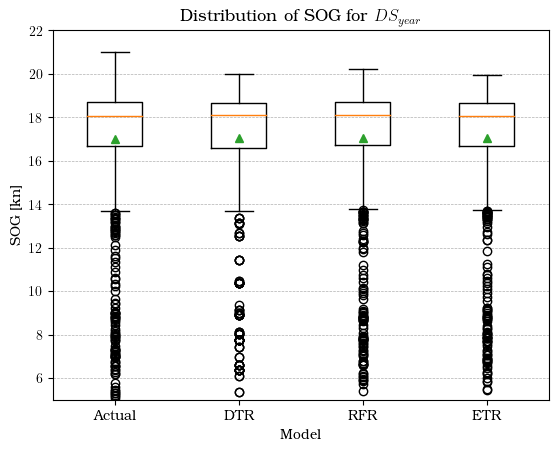
\includegraphics[width=\textwidth]{02_figures/sog_pred_year.png}
    % \caption{Caption for Picture 1.}
    \label{fig:boxplot_dsyear}
\end{minipage}%
\hfill
\begin{minipage}[b]{0.32\textwidth}
    \centering
    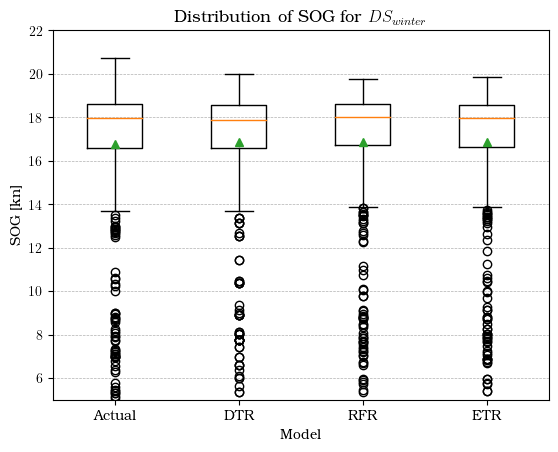
\includegraphics[width=\textwidth]{02_figures/sog_pred_winter.png}
    % \caption{Caption for Picture 2.}
    \label{fig:boxplot_dswinter}
\end{minipage}%
\hfill
\begin{minipage}[b]{0.32\textwidth}
    \centering
    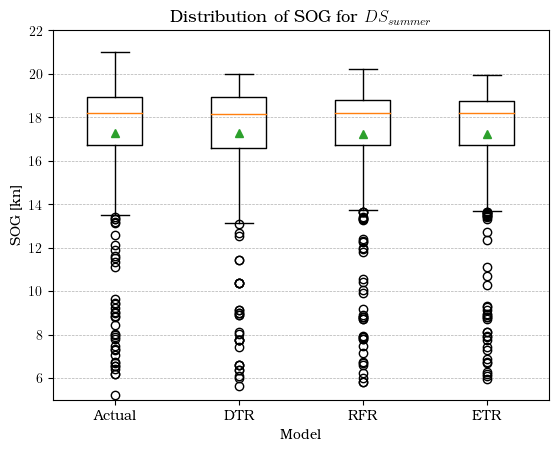
\includegraphics[width=\textwidth]{02_figures/sog_pred_summer.png}
    % \caption{Caption for Picture 3.}
    \label{fig:boxplot_dssummer}
\end{minipage}

\caption{SOG distribution for $DS_{year}$, $DS_{winter}$ and $DS_{summer}$}
\label{fig:boxplot_sogPred_overall}
\end{figure}  

To gain more insight to the predictive performance, descriptive statistics of the SOG prediction is provided \Cref{tbl:SOG_pred_descriptive}. The results implied that the model is not able to capture information on the lower end of the ship speed across the different datasets. This is possibly caused by low number of data points that represent lower end of the SOG speed, this is evident from the boxplots of the different datasets shown in \Cref{fig:boxplot_sogPred_overall} and the plot actual against predicted SOG shown in \Cref{fig:pred_vs_act_SOG}. The sparsity of data points in lower SOG range is clearly indicated in \Cref{fig:pred_vs_act_SOG}.\\

\begin{figure}[h]
    \centering
        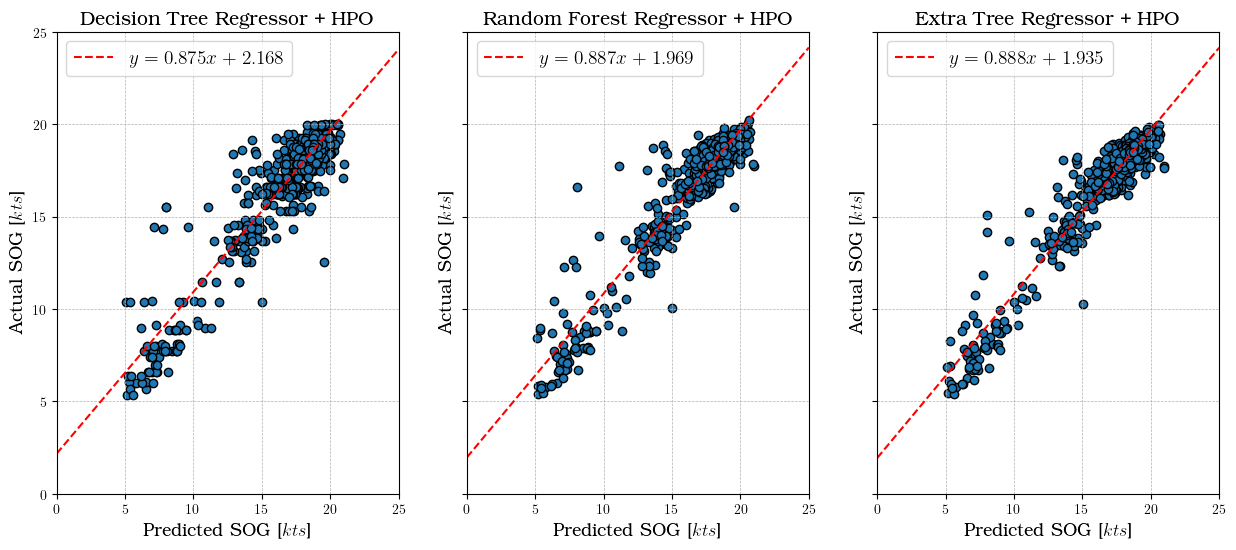
\includegraphics[width=.9\textwidth]{02_figures/pred_vs_act_all_tree.png}
        \caption{Actual vs Predicted SOG for DTR, RFR and ETR}
        \label{fig:pred_vs_act_SOG}
\end{figure}

Both the descriptive statistics and boxplots implied that the data points distributions are skewed towards the higher end of SOG, with the majority of data points concentrated within approximately 16.5 knots for the first quartile and 19 knots for the third quartile across all datasets. The lowest data point within the $1.5 \cdot \text{IQR}_{LOW}$ distribution lies at approximately 13.6 knots, which is indicated by the lower whisker in the boxplot. Although the boxplots may suggest that data points beyond the whisker are outliers, this is not the case, as these points should represent ship journeys at low speeds. The limited representation of low-speed data points contributes to the model's inability to effectively predict SOG at the lower end of the range.\\

This may explain the relatively high value of RMSE for all models as it treats the data points for low SOG as outliers, as previously discussed in \Cref{sec:perf_metrics}, RMSE are more sensitive to outliers in comparison to both MAE and MAD, making it less representative in this case study which results in MAE and MAD being the more suitable error evaluation metrics to be used in this case study. Furthermore, the high scores of $R^2$ and explained Variance can be attributed to the models' ability to predict SOG values that lie within the whiskers of the box plots, indicating good prediction performance within those ranges.\\

There are two possible solutions to address this problem:\\ 

\textbf{Increasing the number of data points in lower SOG range}: this is the apparent solution to this problem, this will help widen the IQR of the boxplot, and it should not misclassify data points in lower range of the SOG as outliers. This could also potentially improve the results of performance indices such as $R^2$ and RMSE. However, \emph{specific to this case study}, this may not be possible as the limitation of T-AIS shown in \Cref{fig:aiscoverage}. The ship will decrease its speed as it approach a port, or it will gradually increase its speed as it leaves a port. However, T-AIS coverage around the port of K{\o}ge and R{\o}nne are either problematic i.e. transmission reception rate at around $50\%$ to $80\%$ or poor i.e. transmission rate less than $50\%$. This may prove to be challenging to as it may not be possible to increase the number of data points around these regions.\\ 

\textbf{Reducing skew of the data}: \bcitet{Gkerekos.2019} applied the outlier rejection formula which uses the formula $\mu \pm 3\sigma$, where $\mu$ is the mean and $\sigma$ is the standard deviation. Assuming normal distribution, $99.7\%$ of the normal data should be within this range. Another method of reducing the skew is by applying higher threshold of the minimum SOG value. While this may help reduce overall errors and improve model fit, this approach will negate the capability of the model to make prediction when the ship is sailing at a reduced speed. Careful consideration of the trade-offs is required when selecting the most appropriate approach.\\

\section{Evaluation of WBM}\label{sec:WBM_perf_eval}

\subsection{Analysis of WBM}\label{sec:Power_estimation_actual}

The findings of power estimation using the Holtrop-Mennen method are presented in \Cref{tbl:PB_act_descriptive_yr} and \Cref{fig:hist_resistance_power_yr}. To gain insights into the overall model behavior, the analysis is conducted using the actual data from the $DS_{year}$ datasets.To facilitate a better interpretation of the scale of magnitude, the histograms for the resistance components utilize identical scaling.\\

For calm water resistance $R_{CALM}$, the largest portion is attributed to the frictional resistance $R_F$, which accounts for approximately $39\%$ of $R_{TOTAL}$ when considering the mean. Following this, the wave-making and breaking resistance $R_W$ contribute around $21\%$. Subsequently, the bulbous bow resistance $R_{B}$ accounts for approximately $16\%$, the correlation resistance $R_{A}$ around $10\%$, and the appendage resistance $R_{APP}$ at approximately $8\%$. The transom resistance $R_{TR}$ has a relatively negligible impact on $R_{CALM}$, accounting for only about $1\%$.\\

Reagrding the added resistance due to surrounding weather conditions, the contribution of added resistance due to wind $R_{AA}$ are noticeable and add a significant amount to the total resistance $R_{TOTAL}$. In contrast, the added resistance due to waves $R_{AW}$ is comparatively negligible. This behavior can be explained by referring to \Cref{tbl:testyear_dataset_descriptive}, the sea conditions along the ship's sailing path are relatively calm, with a mean significant wave height $H_{1/3}$ of $0.77 m$ and a mean wind speed of $6.45 m/s$. By only considering the mean, the combined additional resistance to weather conditions only makes up to about $3.5\%$ of the total resistance.\\

These results further validate the BBM's ranking of ship draught $T$ as the most significant physical factor that affect the ship speed. The WBM also further confirm the BBM suggestion that wave resistance might have a more significant impact on the speed compared to wind resistance. This is evident from the maximum achievable resistance of $R_{AA}$ and $R_{AWL}$ shown in \Cref{tbl:PB_act_descriptive_yr}. However, over the journey, the mean of $R_{AWL}$ is significantly lower, primarily due to the condition in \Cref{eqn:stawave1}, which only consider the wave correction force within $\pm 45$° off bow.\\  

\begin{table}[h]
    \footnotesize
    \centering
    % \resizebox {\textwidth}{!}
    {\begin{tabular}{ p{0.04\linewidth} p{0.03\linewidth} c c c c c c c c }
    \hline
    Features && Count & Mean & std & Min & 25\% & 50\% & 75\% & Max \\
    \hline
    $STW$ & $[kt]$ & 957.00 &  17.03 &  3.10 &  5.14 &  16.62 &  18.07 &  18.79 &  21.08 \\
    $R_F $&$[kN]$ & 957.00 & 174.65 & 49.25 & 17.17 & 162.08 & 189.16 & 205.18 & 262.25 \\
    $R_{APP} $&$[kN]$ & 957.00 &  39.52 &  11.29 &  3.64 &  36.53 &  43.03 &  46.46 &  58.25 \\
    $R_{W} $&$[kN]$ & 957.00 &  96.51 &  55.49 &  0.00 &  61.08 & 102.36 & 129.98 & 297.53 \\
    $R_{B} $&$[kN]$& 957.00 &  71.23 &  11.30 & 15.59 &  69.79 &  74.93 &  77.64 &  82.20 \\
    $R_{TR} $&$ [kN]$ & 957.00 &   5.58 &  11.60 &  0.00 &   0.00 &   0.00 &   4.70 &  53.56 \\
    $R_{A} $&$ [kN]$ & 957.00 &  44.45 &  12.85 &  3.92 &  41.03 &  48.37 &  52.44 &  66.23 \\
    $R_{AA}$&$ [kN]$ & 957.00 &  12.15 &  11.27 &  0.01 &   3.07 &   8.74 &  18.08 &  59.50 \\
    $R_{AWL}$&$ [kN]$ & 957.00 &    3.48 &   11.23 &   0.00 &    0.00 &    0.00 &    1.17 &   116.18 \\
    $R_{TOT}$&$ [kN]$ & 957.00 &  447.57 &  129.17 & 100.29 &  387.05 &  473.26 &  527.77 &   784.72 \\
    $\eta_{TOT}$&$ [\%]$ & 957.00 &   0.67 &   0.00 &  0.67 &   0.67 &   0.67 &   0.67 &   0.67 \\
    $P_{B} $&$[kW]$ & 957.00 & 6173.34 & 2361.10 & 397.02 & 4987.21 & 6607.35 & 7654.90 & 12755.90 \\
    \hline
    \textbf{FOC}&$[T/h]$ & 957.00 &   1.04 &   0.40 &  0.06 &   0.84 &   1.11 &   1.29 &   2.09 \\
    \hline
    \end{tabular}}
\caption{Descriptive statistics of Power estimation method}\label{tbl:PB_act_descriptive_yr}
\end{table}

\begin{figure}[h!]
    \centering
    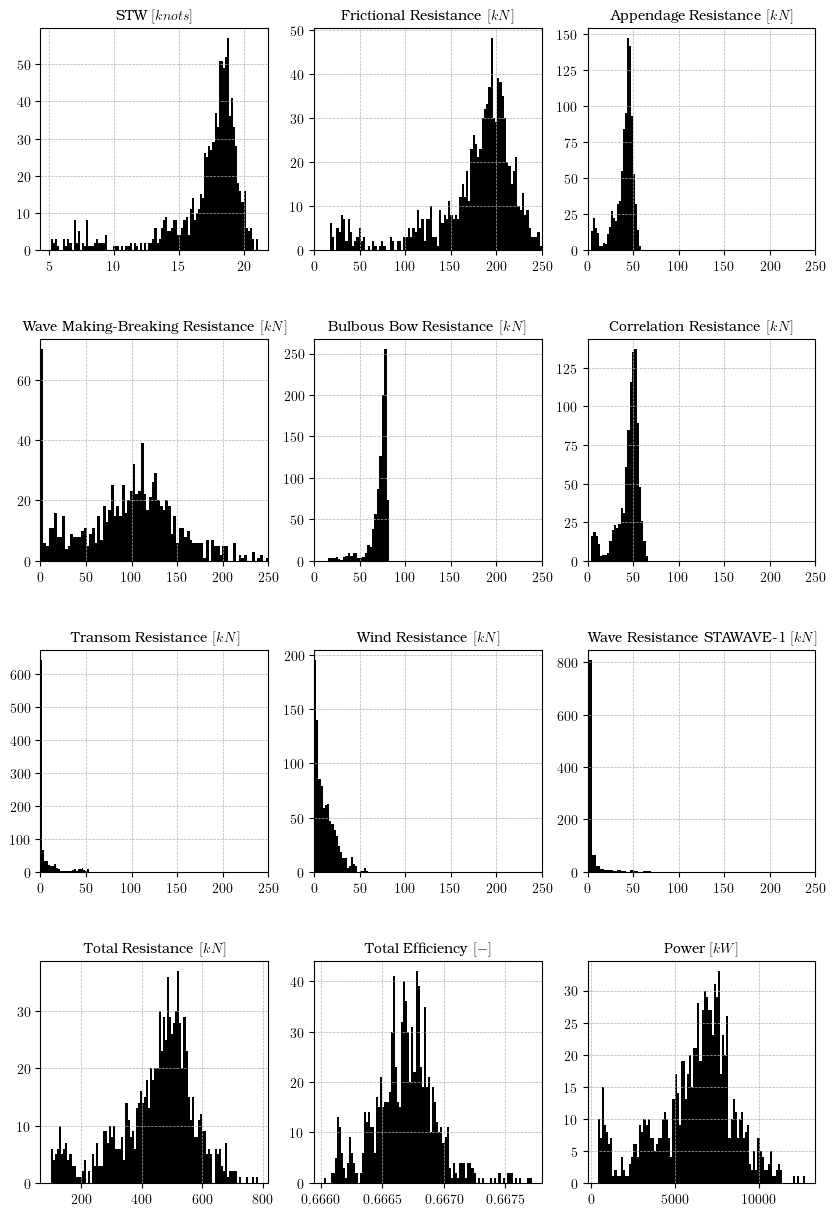
\includegraphics[width=.9\linewidth]{02_figures/resistance_power_hist.png}
    \caption{Histogram of encountered resistances for $DS_{year}$}
    \label{fig:hist_resistance_power_yr}
\end{figure}

By considering the total resistance $R_{TOTAL}$ and the total efficiencies $\eta_{TOTAL}$, the brake power $P_B$ can be calculated. Using the brake power and the corresponding speeds, a power-to-speed curve can be plotted. This curve can then be transformed into a bunker-to-speed curve, which enables the estimation of the energy required for different operating speeds.\\ 

To determine the best regression fit, different polynomial regression lines with varying orders are considered. The selection of the best model is based on the highest $R^2$ score and the ability to minimize the Mean Squared Error (MSE). Similar to BBM, the data is split into training and test sets for model evaluations. The evaluations shows that a polynomial regression fit of order $n=4$ is adequate to fit the data effectively. This model achieves $R^2$ score of $99.92\%$. From \Cref{fig:polyfit_best_MSE}, it can be observed that there is no substantial improvement in performance by increasing the order from $n=4$ to $n=5$.\\

\begin{figure}
    \begin{minipage}{0.35\linewidth} % Adjust the width as needed
      \footnotesize
      \centering
      \begin{tabular}{c c}
          \hline
          Polynomial Order & $R^2$ \\
          $n$&$[\%]$\\
          \hline
            1 & 89.04\\
            2 & 99.29\\
            3 & 99.87\\
            4 & 99.92\\
            5 & 99.93\\
          \hline
      \end{tabular}
    %   \caption{$R^2$ of different polynomial order}
      \label{tbl:polyfit_best_rsquared}
    \end{minipage}
    \hspace{0.01\linewidth}
  %   \hfill
    \begin{minipage}{0.6\linewidth} % Adjust the width as needed
        \centering
        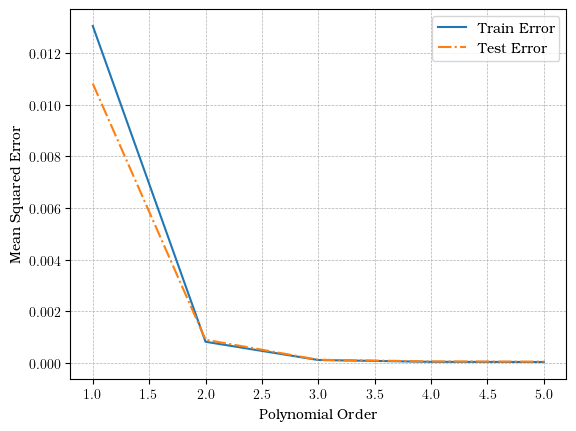
\includegraphics[width=\linewidth]{02_figures/MSE_polyfitplot.png}
        % \caption{MSE plot of different polynomial orders}
        \label{fig:polyfit_best_MSE}
        \end{minipage}
  \caption{Performance indices for different polynomial orders}
  \end{figure}

The resulting plot is shown in figure \Cref{fig:FOC_plot_act_yr}, This resulting bunker to fuel function aligns with the findings from \bcitet{Psaraftis.2013}. The cubic law dictates that the fuel consumption rate can be defined with a propotional factor and saling speed raised to the power of $\alpha = 3$ \bcitep{Du.2019}. However, \bcitet{Psaraftis.2013} stated that the cubic law are not applicable for low speeds, and the the factor $\alpha$ can be 4 or 5 or posssibly even higher for some type of ships or when travelling at high speeds.\\ 

\begin{figure}
    \centering
    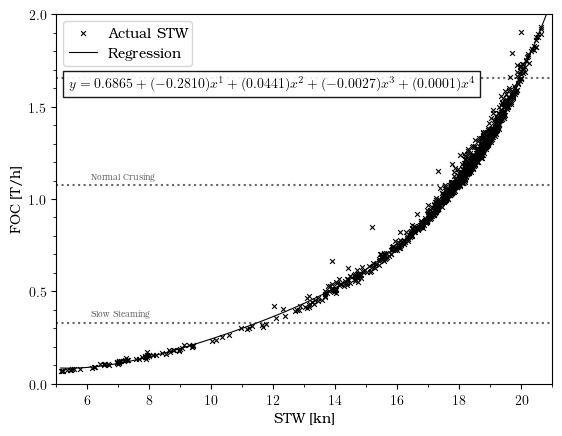
\includegraphics[width=.7\linewidth]{02_figures/FOC_plot_act_yr.png}
    \caption{Bunker-to-speed curve for $DS_{year}$}
    \label{fig:FOC_plot_act_yr}
\end{figure}

However, the observations from \Cref{fig:polyfit_best_MSE} indicate that the improvement in function fit performance is negligible. There is no significant decrease in the MSE, and the attained $R^2$ score of $99.87\%$ shows little variation to the best fit model. Since the model is primarily used to define the ship journey at steady sailing state i.e. at normal operating speed, the limitations of cubic law mentioned by \bcitet{Psaraftis.2013} may not be applicable.\\

The results also indicate that the model predicted ship speeds exceeding the maximum engine rating, which is physically impossible. This issue can be attributed to the conversion of SOG to STW. Analysing the openly accessible data from the research by \bcitet{JoanPeturPetersen.2011}\footnote{\url{http://cogsys.imm.dtu.dk/propulsionmodelling/}}, a noticeable difference between SOG and STW can be observed, typically by a factor of aprroximately 0.85. In this case study, even after current correction, the difference in speed are minimal.\\ 

This suggests that the conversion of SOG and STW should also account the effect of speed loss due to wind and waves. \bcitet{Molland.2017} demonstrated typical speed loss curves based on different Beaufort scales, as shown in \Cref{fig:molland17_speedloss_windwave}. \bcitet{Molland.2017} then presented two formulae by \bcitet{Aertssen.1975} and \bcitet{kwon.2008} for estimating speed loss due to wind and wave effects. However, these formulae have a limited application range and are not optimised for different types of vessels. As a result, these formulae are not implemented in this thesis.\\ 

\begin{figure}
    \centering
    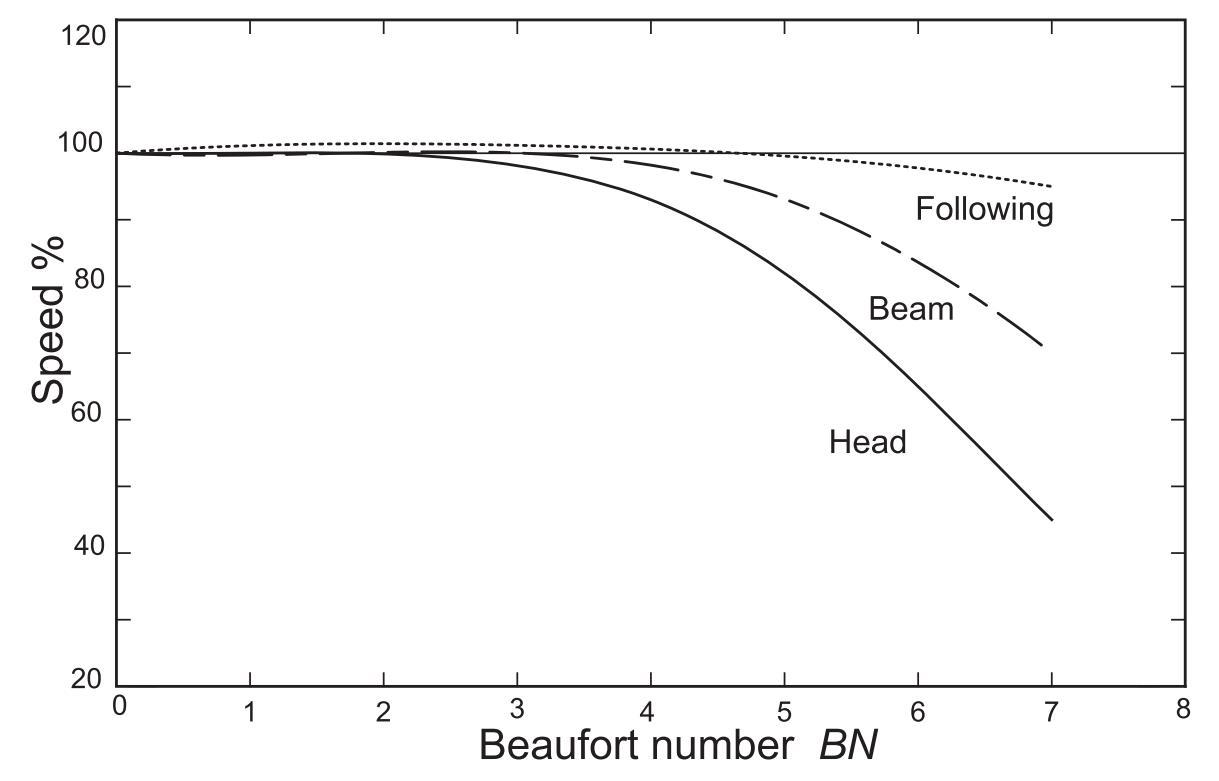
\includegraphics[width=.7\linewidth]{02_figures/molland17_speedlosscurve.jpg}
    \caption{Speed loss with increase in Beaufort Number BN \bcitep{Molland.2017}}
    \label{fig:molland17_speedloss_windwave}
\end{figure}


\subsection{Result and Discussion of WBM}\label{sec:WBM_result_discussion}

\Cref{tbl:FOC_scores_errors} present the results for FOC prediction for different modelling approches and datasets. ETR model shows best perfomance followed by RFR and DTR, the similarity in the results can be attributed to the sequential approach of GBM. The output from the BBM is used as the input for WBM as shown in \Cref{fig:flowchart_GBM}. Decline in $R^2$ score, explained variance and MAPE performance across all models is also observed.\\ 

This decrease in performance may be caused due to the nonlinearity of the WBM, which magnifies FOC prediction error at higher ship speed. This behaviour is demosntrated through the case study by \bcitet{Birk.2019} shown in \Cref{fig:birk19_Pb_nonlinear}. At the lower end of the ship speed, a difference of $1$ knot resulted in a power difference of approximately $1200$ kW. However, at the higher end of the ship speed, the power difference increases to about $2300$ kW. Assuming that the engine in \bcitet{Birk.2019} case study has the identical SFOC as the engine in this thesis, this translates to FOC differences of approximately $0.2$ T/h and $0.4$ T/h, respectively.\\

\begin{table}[h]
    % \footnotesize
    \small
    \centering
    % \resizebox {\textwidth}{!}
    {\begin{tabular}{ l l c c c c c c }
    \hline
    Model & Dataset & $R^2$ & expVar & MAE & RMSE & MAD & MAPE \\
    & & [$\%$] & [$\%$] & [$T/h$] & [$T/h$] & [$T/h$] & [$\%$]  \\ 
    \hline
    $\text{DTR}_{OPT}$ & $DS_{year}$ & 76.59 & 76.63 & 0.133 & 0.193  & 0.087 & 15.79  \\
    & $DS_{winter}$ & 78.24 & 78.25 & 0.123 & 0.179 & 0.080 & 15.38 \\
    & $DS_{summer}$ & 74.42 & 74.73 & 0.145 &  0.208 & 0.096 & 16.25 \\
    $\text{RFR}_{OPT}$ & $DS_{year}$  & 81.82 & 81.89 & 0.117 & 0.170 & 0.079 & 13.65 \\
    & $DS_{winter}$ & 86.55 & 86.56 & 0.099 & 0.141 & 0.069 & 12.08 \\
    & $DS_{summer}$ & 76.81 & 77.20 & 0.137 & 0.198 & 0.088 & 15.37 \\
    $\text{ETR}_{OPT}$ & $DS_{year}$ & 83.84 & 84.01 & 0.111 & 0.161 & 0.076 & 12.45\\
    & $DS_{winter}$ & \textbf{87.57} & \textbf{87.57} & \textbf{0.097} & \textbf{0.135} & \textbf{0.068} & \textbf{11.37} \\
    & $DS_{summer}$ & 79.86 & 80.49 & 0.127 & 0.184 & 0.082 & 13.64 \\
    MLR & $DS_{year}$ & 29.34 & 32.03 & 0.223 & 0.336 & 0.171 & 29.35 \\
    & $DS_{winter}$ & 11.98 & 13.09 & 0.212 & 0.360 &0.162& 33.02 \\
    & $DS_{summer}$ & 44.28 & 49.44 & 0.235 & 0.307 & 0.191 & 25.29 \\
    \hline
    \end{tabular}}
\caption{Performance indices for FOC prediction}\label{tbl:FOC_scores_errors}
\end{table}

\begin{figure}
    \centering
    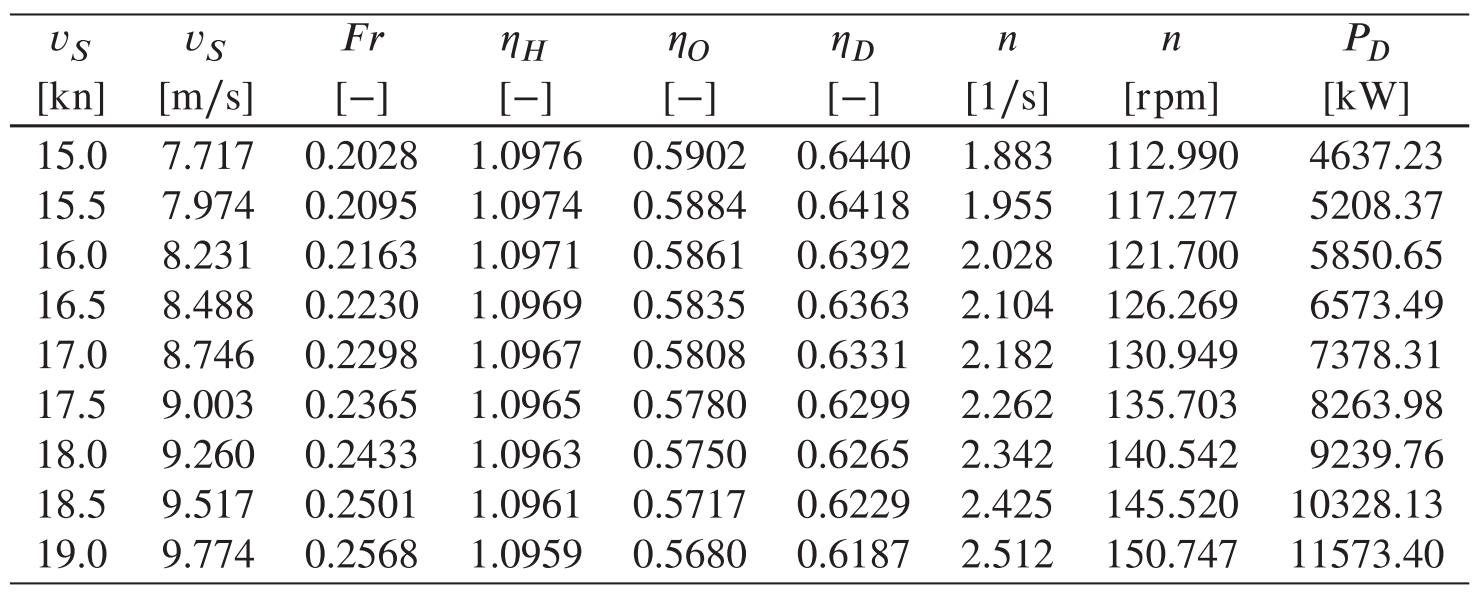
\includegraphics[width=.8\linewidth]{02_figures/birk19_Pb_nonlinear_case.jpg}
    \caption{Case study for power estimation by \bcitet{Birk.2019}}
    \label{fig:birk19_Pb_nonlinear}
\end{figure}

This may also explain the inability of the model to accurately predict FOC for higher speeds. As shown in \cref{fig:foc_etr_rfr_yr} and \cref{fig:foc_dtr_mlr_yr}. The plots also indicated the underfitting behavior of the generated model. Nevertheless, the prediction errors of the model is reasonable, taking the example of the $DS_{year}$ the MAE ranges between $0.111$ T/h to $0.133$ T/h for mean FOC of $1.04$ T/h. Overall, the pred\\

\begin{figure}
    \centering
    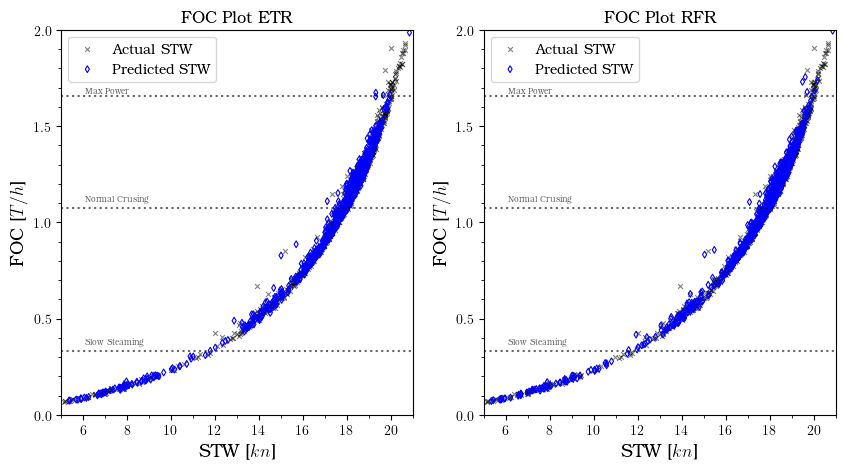
\includegraphics[width=.9\linewidth]{02_figures/FOC_act_pred_etr_rfr.png}
    \caption{Predicted and Actual FOC for ETR and RFR using $DS_{year}$}
    \label{fig:foc_etr_rfr_yr}
\end{figure}

\begin{figure}
    \centering
    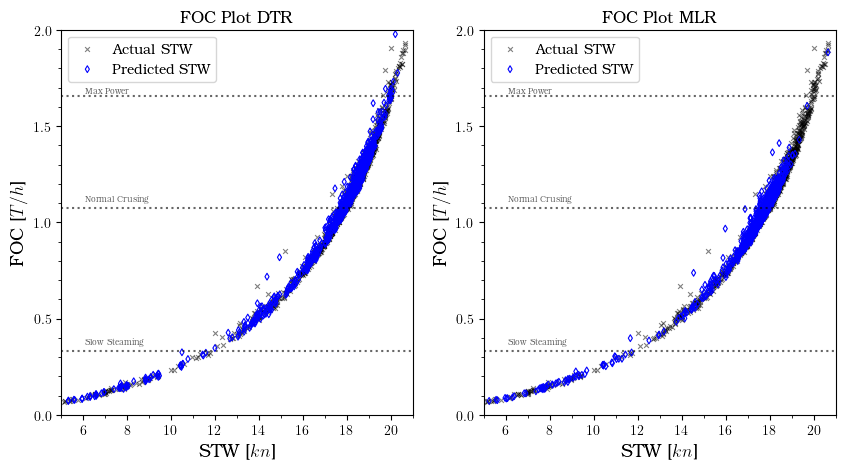
\includegraphics[width=.9\linewidth]{02_figures/FOC_act_pred_dtr_mlr.png}
    \caption{Predicted and Actual FOC for DTR and MLR using $DS_{year}$}
    \label{fig:foc_dtr_mlr_yr}
\end{figure}

To evaluate the accuracy and precision of the generated bunker-to-speed function, the best regression fit for the predicted FOC will be compared against the regression fit of the actual case. The test data used for this evaluation will be random generated values between $5$ knots to $21$ knots with different STW distribution compared to the STW distribution used to generate the best fit regression line. The distribution of the test data is presented in \cref{fig:hist_dummy_test} and the results is summarised in 

\begin{figure}
    \centering
    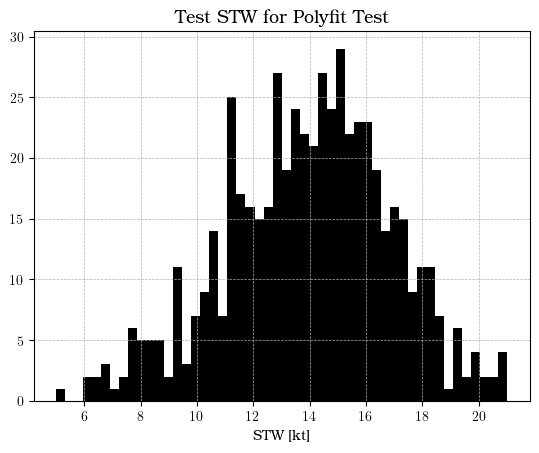
\includegraphics[width=.6\linewidth]{02_figures/hist_dummy_stw.png}
    \caption{STW ditribution for regression test}
    \label{fig:hist_dummy_test}
\end{figure}

\begin{table}[h]
    % \footnotesize
    \small
    \centering
    % \resizebox {\textwidth}{!}
    {\begin{tabular}{ l l c c c c c c }
    \hline
    Model & Dataset & $R^2$ & expVar & MAE & RMSE & MAD & MAPE \\
    & & [$\%$] & [$\%$] & [$T/h$] & [$T/h$] & [$T/h$] & [$\%$]  \\ 
    \hline
    $\text{DTR}_{OPT}$ & $DS_{year}$ & 76.59 & 76.63 & 0.133 & 0.193  & 0.087 & 15.79  \\
    & $DS_{winter}$ & 78.24 & 78.25 & 0.123 & 0.179 & 0.080 & 15.38 \\
    & $DS_{summer}$ & 74.42 & 74.73 & 0.145 &  0.208 & 0.096 & 16.25 \\
    $\text{RFR}_{OPT}$ & $DS_{year}$  & 81.82 & 81.89 & 0.117 & 0.170 & 0.079 & 13.65 \\
    & $DS_{winter}$ & 86.55 & 86.56 & 0.099 & 0.141 & 0.069 & 12.08 \\
    & $DS_{summer}$ & 76.81 & 77.20 & 0.137 & 0.198 & 0.088 & 15.37 \\
    $\text{ETR}_{OPT}$ & $DS_{year}$ & 83.84 & 84.01 & 0.111 & 0.161 & 0.076 & 12.45\\
    & $DS_{winter}$ & \textbf{87.57} & \textbf{87.57} & \textbf{0.097} & \textbf{0.135} & \textbf{0.068} & \textbf{11.37} \\
    & $DS_{summer}$ & 79.86 & 80.49 & 0.127 & 0.184 & 0.082 & 13.64 \\
    MLR & $DS_{year}$ & 29.34 & 32.03 & 0.223 & 0.336 & 0.171 & 29.35 \\
    & $DS_{winter}$ & 11.98 & 13.09 & 0.212 & 0.360 &0.162& 33.02 \\
    & $DS_{summer}$ & 44.28 & 49.44 & 0.235 & 0.307 & 0.191 & 25.29 \\
    \hline
    \end{tabular}}
\caption{Performance indices for FOC regression functions}\label{tbl:polyfit_scores_errors}
\end{table}










